\documentclass[12pt]{article}
\usepackage[utf8]{inputenc}
\usepackage{float}
\usepackage{amsmath}
\usepackage{tikz} % for Hasse diagram
\usepackage[hmargin=3cm,vmargin=6.0cm]{geometry}
%\topmargin=0cm
\topmargin=-2cm
\addtolength{\textheight}{6.5cm}
\addtolength{\textwidth}{2.0cm}
%\setlength{\leftmargin}{-5cm}
\setlength{\oddsidemargin}{0.0cm}
\setlength{\evensidemargin}{0.0cm}

\begin{document}
	
\section*{Student Information } 
%Write your full name and id number between the colon and newline
%Put one empty space character after colon and before newline
Full Name :  Adil Kaan Akan\\
Id Number :  2171155\\

% Write your answers below the section tags
\section*{Answer 1}
In this question, we can have answer by calculating ternary string that not contain three consecutive 0s, 1s and 2s and substracting that from all number of ternary strings. \\
Let $X_n$ be ternary string that not three contain consecutive 0s,1s and 2s. Then, \\
$a_n = 3^n - X_n$ \\
$X_n = {X0}_n+{X1}_n+{X2}_n$ where $X0$, $X1$, $X2$ are string that starts with 0, 1, 2 respectively. \\
Think $X0$ that starts with 0. We can have the following options \\
"01..." \\
"02..." \\
"001.." \\
"002.." \\
Realizing that we have recurrence relation in that case such that \\
"01..." is ${X1}_n$ which is ternary string starts with 1 and length n-1 \\
"02..." is ${X2}_n$ which is ternary string starts with 2 and length n-1 \\
"001.." is ${X1}_{n-1}$ which is ternary string starts with 1 and length n-2 \\
"002.." is ${X2}_{n-1}$ which is ternary string starts with 2 and length n-2 \\
Then we have \\
${X0}_n = {X1}_{n-1} + {X2}_{n-1} +{X1}_{n-2} + {X2}_{n-2} $

Similarly, in $X1$ and $X2$ we have \\
In $X1$, \\
"10..." \\
"12..." \\
"110.." \\
"112.." \\
Then, we will have \\
${X1}_n = {X0}_{n-1} + {X2}_{n-1} +{X0}_{n-2} + {X2}_{n-2} $ \\
In $X2$, \\ 
"20..." \\
"21..." \\
"220.." \\
"221.." \\
Then, we will have \\
${X2}_n = {X0}_{n-1} + {X1}_{n-1} +{X0}_{n-2} + {X1}_{n-2} $ \\
If we sum all of these we will have $X_n$ \\
$X_n = {X0}_n+{X1}_n+{X2}_n$ \\
$X_n = {X1}_{n-1} + {X2}_{n-1} +{X1}_{n-2} + {X2}_{n-2}+{X0}_{n-1} + {X2}_{n-1} +{X0}_{n-2} + {X2}_{n-2} +{X0}_{n-1} + {X1}_{n-1} +{X0}_{n-2} + {X1}_{n-2}$ \\
$X_n = 2*({X_0}{n-1}+{X_1}{n-1}+{X_2}{n-1}) +2*({X_0}{n-2}+{X_1}{n-2}+{X_2}{n-2}) $ \\
$X_n = 2* X_{n-1} + 2*X_{n-2}$ \\
$a_n = 3^n - X_n$ \\
$a_{n-1} = 3^{n-1} - X_{n-1}$ \\
$a_{n-2} = 3^{n-2} - X_{n-2}$ \\
If we get $X_n$'s here  \\
$X_n = 3^n - a_n$ \\
$X_{n-1} = 3^{n-1} - a_{n-1}$ \\
$X_{n-2} = 3^{n-2} - a_{n-2}$ \\
$X_n = 2*({X_0}{n-1}+{X_1}{n-1}+{X_2}{n-1}) +2*({X_0}{n-2}+{X_1}{n-2}+{X_2}{n-2}) $
$a_n = 3^n - (2* X_{n-1} + 2*X_{n-2})$ \\
$a_n = 3^n - (2*(3^{n-1} - a_{n-1}) + 2*(3^{n-2} - a_{n-2}))$ \\
If we rearrange the equation we will get \\
$a_n = 3^n - 2*3^{n-1} - 2*3^{n-2} + 2*a_{n-1} + 2*a_{n-2}$ \\
For the base conditions, we have to look the $a_1$, $a_2$ and $a_3$ \\
$a_1 = 0$ since it cannot contain 3 consecutive 0,1 or 2 \\
$a_2 = 0$ since it cannot contain 3 consecutive 0,1 or 2 \\
$a_3 = 3$ where the strings "000","111" and "222"  \\

\section*{Answer 2}
\subsection*{a)}
We can cover $3x1$ board with $2x1$ tiles in 3 ways. First, we can horizontally place $2x1$ tiles. Second, we can use one horizontally and 2 vertically. Third and final, we can use 2 horizontally first and then use vertically. Then we will have, \\

\begin{tabular}{|cccc|}
\hline 
 &  &  & \tabularnewline
 &  &  & \tabularnewline
\hline 
\hline 
 &  &  & \tabularnewline
 &  &  & \tabularnewline
\hline 
\hline 
 &  &  & \tabularnewline
 &  &  & \tabularnewline
\hline 
\end{tabular} \\
First possibility

$ $ \\
$ $ \\

\begin{tabular}{|cc||cc|}
\hline 
 & \multicolumn{1}{c}{} &  & \tabularnewline
 & \multicolumn{1}{c}{} &  & \tabularnewline
\hline 
\hline 
 &  &  & \tabularnewline
 &  &  & \tabularnewline
 &  &  & \tabularnewline
 &  &  & \tabularnewline
\hline 
\end{tabular} \\
Second possibility

$ $ \\
$ $ \\

\begin{tabular}{|cc||cc|}
\hline 
 &  &  & \tabularnewline
 &  &  & \tabularnewline
 &  &  & \tabularnewline
 &  &  & \tabularnewline
\hline 
\hline 
 & \multicolumn{1}{c}{} &  & \tabularnewline
 & \multicolumn{1}{c}{} &  & \tabularnewline
\hline 
\end{tabular} \\
Third possibility

$ $ \\
$ $ \\

\subsection*{b)}
Then, we can use these possibilities such that putting that possibilities at the end of the $3xn$ board. \\
Then, we will have 3 option at the end, and the rest of the board will be $a_{n-2}$ if we think the number of ways to cover $3xn$ board. Since mirrored considered as the same, we should not count them twice. Let x,y,z be first possibility, second possibility and third possibility respectively.Let $a_{n}$ be the number of ways to cover $3xn$ board. Then, $a_2$ is number of ways to cover $3x2$ board. We can do it with three possibility. However, second and third possibility are mirror image of each other and we should not count both of them. Then, there is two way which are first possibility and second possibility and we can show them by x or y. For $a_4$ which is $3x4$, we will put the possibilities at the end of the $a_2$. Then, we can make these possibilities \\
after first possibility we can put three possibility and after second possibility we can put three possibility. Then, we will have \\
x,x \\
x,y \\
x,z \\
y,x \\
y,y \\
y,z \\
Since y and z are mirror image of each other, x,y and x,z are mirror image of each other also and we should not count these twice. \\
Then $a_4$ has 5 possibilities which are \\
x,x \\
x,y \\
y,x \\
y,y \\
y,z \\
For $a_6$ which is $3x6$ board, after putting three possibilities after the $a_4$, we will have \\
x,x,x \\
x,x,y \\
x,x,z \\
x,y,x \\
x,y,y \\
x,y,z \\
y,x,x \\
y,x,y \\
y,x,z \\
y,y,x \\
y,y,y \\
y,y,z \\
y,z,x \\
y,z,y \\
y,z,z \\
Realizing that only x,x,y and x,x,z are mirror image of each other and there is no other mirror image. \\
We can easily conclude that in every step we will have just one mirror image. Therefore, we can generalize the $a_n$ by \\
$a_n = 3*a_{n-2} - \frac{(-1)^n + 1}{2}$ and $a_0=0$ and $a_1=0$ \\ we have the term $(-1)^n + 1$ because we need odd terms to be zero since we cannot cover $3x(odd number)$ board with $3x2$ tiles and we need to substract 1 because of the mirror images.
\subsection*{c)}
$a_n = 3*a_{n-2} - \frac{(-1)^n + 1}{2}$ \\
Assume that $<a_0,a_1,a_2,a_3,a_4,a_5,....,a_n,...> \Longleftrightarrow A(x)$ \\
Then, we will have \\
\begin{align*}
A(x) &= 2x^2 + \sum\limits_{n=3}^{\infty} a_n*x^n \\
&=2x^2 + \sum\limits_{n=3}^{\infty}(3*a_{n-2} - \frac{(-1)^n + 1}{2})*x^n \\
&= 2x^2 + \sum\limits_{n=3}^{\infty}(3*a_{n-2})*x^n - \sum\limits_{n=3}^{\infty}\frac{(-1)^n + 1}{2}*x^n \\
A(x) &= 2x^2 + 3x^2*\sum\limits_{n=3}^{\infty}a_{n-2}*x^n - x^4*(1+x^2+x^4+x^6+x^8+x^10+....) \\
&=2x^2+x^2*A(x) - x^4(\frac{1}{1-x^2}) \\
A(x) &= \frac{2x^2-3x^4}{1-x^2}*\frac{1}{1-3x^2} \\ 
A(x) &= \frac{1}{2}*\frac{1}{1-x^2}+\frac{1}{2}*\frac{1}{1-3x^2} - 1 \\
\end{align*}

$\frac{1}{2}*\frac{1}{1-x^2} = \frac{1}{2}*(1+x^2+x^4+x^6+x^8+x^10+....)$ which is $<\frac{1}{2},0,\frac{1}{2},0,\frac{1}{2},0,...,\frac{(-1)^n + 1}{2}*\frac{1}{2},.,>$ \\

$\frac{1}{2}*\frac{1}{1-3x^2} = \frac{1}{2} * (1+3x^2+3^2x^4+3^3+x^6,....)$ which is $<\frac{1}{2},0,\frac{1}{2}*3,0,\frac{1}{2}*3^2,0,\frac{1}{2}*3^3,0,.,\frac{(-1)^n + 1}{2}*\frac{3^{\frac{n}{2}}}{2},...>$ \\
and \\
$1 = <1,0,0,0,0,0,0,...>$ \\
If we sum all of them, we will get \\
$A(x) = <0,2,0,5,....,\frac{(-1)^n + 1}{2}*(\frac{1}{2}+\frac{3^{\frac{n}{2}}}{2}),....>$ \\
Then, $a_n = \frac{(-1)^n + 1}{2}*(\frac{1}{2}+\frac{3^{\frac{n}{2}}}{2})$





\section*{Answer 3}
If a relation,R, is partial ordering on set,S, then, it is reflexive, 
antisymmetric, and transitive.
\subsection*{a)}
For reflexivity, we can say that for set U, we need $U \subseteq U$ and $U \subseteq U$. This means that U=U and that is always true. Therefore, we can say that the set inclusion is reflexive for every set. \\
For transitivity, for sets U,V and W we need to show , if $U \subseteq V$ and $V \subseteq W$, then $U \subseteq W$. The $U \subseteq V$ means that for every x, if $x\in U$, then $x \in V$ and similarly, The $v \subseteq W$ means that for every x, if $x\in V$, then $x \in W$. Let a be the arbitrary element of U and then, we know that x is element of V by definition of subset relation.Likewise, since x is element of V, then, x is element of W also. Since x is arbitrary element of U and W by definition, then we can say that that is true for every element of U. Then, we can say that the relation is transitive. \\
For antisymmetricity, to be antisymmetric, we need to show if  $U \subseteq V$ and $V \subseteq U$, then $U=V$ must be true. That is definition of  set equality and that is true for every set U and V. We can say that the relation is antisymmetric.
Since set inclusion relation has reflexivity, transitivity and antisymmetricity, we can say that it is partial ordering on set of integers \textbf{Z}.
\subsection*{b)}
Assume that the divides relation is partial ordering on set of integer \textbf{Z}. Then,  it must have reflexivity, transitivity and antisymmetricity by definition of partial ordering. For antisymmetricity, we need to show that for every a and b, if $a|b$ and $b|a$, then $a=b$. Assume that $b = - a$ , and we have $a|b$ and $b|a$ that are true. However, $a\neq b$. That is contradiction and our assumption is wrong. We have disprove this by contradiction. \\
\subsection*{c)}
For reflexivity, we can show that by r=1, then, $a=a^1$. The relation is reflexive. \\
For transitivity, we need to show $aRb \land bRc \implies aRc$. We can show that by $b = a^r$ and $c = b^t$, then we can gather them into $c=a^{rx}$ and $a,c \in \textbf{Z}$.Therefore, we can say that the relation is transitive. \\
For antisymmetricity, we need to show that $aRb \land bRa \implies a=b$. Then we can show that by $b=a^r$, $a=b^x$, then $a=a^{rx}$. By the given condition x and r are positive integers. We know that $rx = 1$ since $a= a^{rx}$. Then, $r=1$ and $x=1$,  then we can say that the given relation is antisymmetric. 
Since set given relation has reflexivity, transitivity and antisymmetricity, we can say that it is partial ordering on set of integers.


\section*{Answer 4}
\subsection*{a)}
There are 7 partitions of 5 such that \\
$1+1+1+1+1  = 5$ \\
$1+1+1+2  = 5$ \\
$1+2+2 = 5$ \\
$1+1+3 = 5$ \\
$2+3 = 5$ \\
$1+4 = 5$ \\
$5 = 5$ \\

$ $\\
$ $\\
$ $\\
$ $\\
The set partion is \\
$P = (
(1,1,1,1,1)$, \\
$(1,1,1,2)$, \\
$(1,2,2)$, \\
$(1,1,3)$, \\
$(2,3)$, \\
$(1,4)$, \\
$(5) )$ \\

\subsection*{b)}
%Hasse diagram example
\begin{figure}[H]
\centering
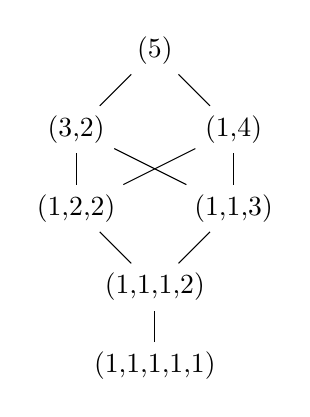
\begin{tikzpicture}
%%   kw   (name)   (x, y)   {text}
    \node (lt1) at (2, 4)     {(5)};
    \node (md1) at (3, 3)    {(1,4)};
    \node (lt2) at (1, 3)     {(3,2)};
    \node (rt2) at (3, 2)     {(1,1,3)};
    \node (lt3) at (1, 2)     {(1,2,2)};
    \node (rt3) at (2,1)     {(1,1,1,2)};
	\node (md4) at (2, 0)     {(1,1,1,1,1)};

    \draw (md4) -- (rt3);
    \draw (rt3) -- (lt3);
    \draw (rt3) -- (rt2);
    \draw (rt2) -- (lt2);
    \draw (lt3) -- (lt2);
    \draw (lt3) -- (md1);
    \draw (rt2) -- (md1);
    \draw (md1) -- (lt1);
    \draw (lt2) -- (lt1);
\end{tikzpicture} \caption{Diagram of partitions of 5}
\end{figure}

\end{document}